\documentclass[]{article}
\usepackage{lmodern}
\usepackage{amssymb,amsmath}
\usepackage{ifxetex,ifluatex}
\usepackage{fixltx2e} % provides \textsubscript
\ifnum 0\ifxetex 1\fi\ifluatex 1\fi=0 % if pdftex
  \usepackage[T1]{fontenc}
  \usepackage[utf8]{inputenc}
\else % if luatex or xelatex
  \ifxetex
    \usepackage{mathspec}
  \else
    \usepackage{fontspec}
  \fi
  \defaultfontfeatures{Ligatures=TeX,Scale=MatchLowercase}
\fi
% use upquote if available, for straight quotes in verbatim environments
\IfFileExists{upquote.sty}{\usepackage{upquote}}{}
% use microtype if available
\IfFileExists{microtype.sty}{%
\usepackage{microtype}
\UseMicrotypeSet[protrusion]{basicmath} % disable protrusion for tt fonts
}{}
\usepackage[margin=1in]{geometry}
\usepackage{hyperref}
\hypersetup{unicode=true,
            pdftitle={Atlas-PS 5},
            pdfauthor={David Atlas},
            pdfborder={0 0 0},
            breaklinks=true}
\urlstyle{same}  % don't use monospace font for urls
\usepackage{color}
\usepackage{fancyvrb}
\newcommand{\VerbBar}{|}
\newcommand{\VERB}{\Verb[commandchars=\\\{\}]}
\DefineVerbatimEnvironment{Highlighting}{Verbatim}{commandchars=\\\{\}}
% Add ',fontsize=\small' for more characters per line
\usepackage{framed}
\definecolor{shadecolor}{RGB}{248,248,248}
\newenvironment{Shaded}{\begin{snugshade}}{\end{snugshade}}
\newcommand{\KeywordTok}[1]{\textcolor[rgb]{0.13,0.29,0.53}{\textbf{{#1}}}}
\newcommand{\DataTypeTok}[1]{\textcolor[rgb]{0.13,0.29,0.53}{{#1}}}
\newcommand{\DecValTok}[1]{\textcolor[rgb]{0.00,0.00,0.81}{{#1}}}
\newcommand{\BaseNTok}[1]{\textcolor[rgb]{0.00,0.00,0.81}{{#1}}}
\newcommand{\FloatTok}[1]{\textcolor[rgb]{0.00,0.00,0.81}{{#1}}}
\newcommand{\ConstantTok}[1]{\textcolor[rgb]{0.00,0.00,0.00}{{#1}}}
\newcommand{\CharTok}[1]{\textcolor[rgb]{0.31,0.60,0.02}{{#1}}}
\newcommand{\SpecialCharTok}[1]{\textcolor[rgb]{0.00,0.00,0.00}{{#1}}}
\newcommand{\StringTok}[1]{\textcolor[rgb]{0.31,0.60,0.02}{{#1}}}
\newcommand{\VerbatimStringTok}[1]{\textcolor[rgb]{0.31,0.60,0.02}{{#1}}}
\newcommand{\SpecialStringTok}[1]{\textcolor[rgb]{0.31,0.60,0.02}{{#1}}}
\newcommand{\ImportTok}[1]{{#1}}
\newcommand{\CommentTok}[1]{\textcolor[rgb]{0.56,0.35,0.01}{\textit{{#1}}}}
\newcommand{\DocumentationTok}[1]{\textcolor[rgb]{0.56,0.35,0.01}{\textbf{\textit{{#1}}}}}
\newcommand{\AnnotationTok}[1]{\textcolor[rgb]{0.56,0.35,0.01}{\textbf{\textit{{#1}}}}}
\newcommand{\CommentVarTok}[1]{\textcolor[rgb]{0.56,0.35,0.01}{\textbf{\textit{{#1}}}}}
\newcommand{\OtherTok}[1]{\textcolor[rgb]{0.56,0.35,0.01}{{#1}}}
\newcommand{\FunctionTok}[1]{\textcolor[rgb]{0.00,0.00,0.00}{{#1}}}
\newcommand{\VariableTok}[1]{\textcolor[rgb]{0.00,0.00,0.00}{{#1}}}
\newcommand{\ControlFlowTok}[1]{\textcolor[rgb]{0.13,0.29,0.53}{\textbf{{#1}}}}
\newcommand{\OperatorTok}[1]{\textcolor[rgb]{0.81,0.36,0.00}{\textbf{{#1}}}}
\newcommand{\BuiltInTok}[1]{{#1}}
\newcommand{\ExtensionTok}[1]{{#1}}
\newcommand{\PreprocessorTok}[1]{\textcolor[rgb]{0.56,0.35,0.01}{\textit{{#1}}}}
\newcommand{\AttributeTok}[1]{\textcolor[rgb]{0.77,0.63,0.00}{{#1}}}
\newcommand{\RegionMarkerTok}[1]{{#1}}
\newcommand{\InformationTok}[1]{\textcolor[rgb]{0.56,0.35,0.01}{\textbf{\textit{{#1}}}}}
\newcommand{\WarningTok}[1]{\textcolor[rgb]{0.56,0.35,0.01}{\textbf{\textit{{#1}}}}}
\newcommand{\AlertTok}[1]{\textcolor[rgb]{0.94,0.16,0.16}{{#1}}}
\newcommand{\ErrorTok}[1]{\textcolor[rgb]{0.64,0.00,0.00}{\textbf{{#1}}}}
\newcommand{\NormalTok}[1]{{#1}}
\usepackage{longtable,booktabs}
\usepackage{graphicx,grffile}
\makeatletter
\def\maxwidth{\ifdim\Gin@nat@width>\linewidth\linewidth\else\Gin@nat@width\fi}
\def\maxheight{\ifdim\Gin@nat@height>\textheight\textheight\else\Gin@nat@height\fi}
\makeatother
% Scale images if necessary, so that they will not overflow the page
% margins by default, and it is still possible to overwrite the defaults
% using explicit options in \includegraphics[width, height, ...]{}
\setkeys{Gin}{width=\maxwidth,height=\maxheight,keepaspectratio}
\IfFileExists{parskip.sty}{%
\usepackage{parskip}
}{% else
\setlength{\parindent}{0pt}
\setlength{\parskip}{6pt plus 2pt minus 1pt}
}
\setlength{\emergencystretch}{3em}  % prevent overfull lines
\providecommand{\tightlist}{%
  \setlength{\itemsep}{0pt}\setlength{\parskip}{0pt}}
\setcounter{secnumdepth}{0}
% Redefines (sub)paragraphs to behave more like sections
\ifx\paragraph\undefined\else
\let\oldparagraph\paragraph
\renewcommand{\paragraph}[1]{\oldparagraph{#1}\mbox{}}
\fi
\ifx\subparagraph\undefined\else
\let\oldsubparagraph\subparagraph
\renewcommand{\subparagraph}[1]{\oldsubparagraph{#1}\mbox{}}
\fi

%%% Use protect on footnotes to avoid problems with footnotes in titles
\let\rmarkdownfootnote\footnote%
\def\footnote{\protect\rmarkdownfootnote}

%%% Change title format to be more compact
\usepackage{titling}

% Create subtitle command for use in maketitle
\newcommand{\subtitle}[1]{
  \posttitle{
    \begin{center}\large#1\end{center}
    }
}

\setlength{\droptitle}{-2em}
  \title{Atlas-PS 5}
  \pretitle{\vspace{\droptitle}\centering\huge}
  \posttitle{\par}
  \author{David Atlas}
  \preauthor{\centering\large\emph}
  \postauthor{\par}
  \predate{\centering\large\emph}
  \postdate{\par}
  \date{9/29/2018}

\usepackage{kbordermatrix}

\begin{document}
\maketitle

\newcommand{\var}{\rm{Var}}
\newcommand{\E}{\rm{E}}





\section{Problem 1}\label{problem-1}

\subsection{a)}\label{a}

We show that \(\var_g{w^*(X)} < M -1\):

\begin{align*}
\var_g{w^*(X)} &= \E[w^*(x)^2] - \E[w^*(x)]^2 \\
&= \E\left[\frac{f(x)^2}{g(x)^2}\right] - \E\left[\frac{f(x)}{g(x)}\right]^2 \\ 
&= \int_{-\infty}^{\infty} \frac{f(x)^2}{g(x)^2} g(x) dx - \int_{-\infty}^{\infty} \frac{f(x)}{g(x)} g(x)dx \\
&= \int_{-\infty}^{\infty}  f(x) \frac{f(x)}{g(x)} dx - \int_{-\infty}^{\infty} f(x)dx.
\end{align*}

Next, we note that \(\frac{f(x)}{g(x)} < M\), by definition and
\(\int_{-\infty}^{\infty} f(x)dx = 1\), as \(f(x)\) is a probability
distribution, which by definition must integrate to 1 over the support.
Therefore, we can write:

\begin{align*}
\int_{-\infty}^{\infty}  f(x) \frac{f(x)}{g(x)} dx - \int_{-\infty}^{\infty} f(x)dx &< \int_{-\infty}^{\infty} M f(x)  dx - 1 \\
&= M \int_{-\infty}^{\infty}f(x)  dx - 1 \\
&= M - 1.
\end{align*}

Therefore, we can say that \(\var_g{w^*(x)} < M -1\).

\subsection{b)}\label{b}

Next, we want to show that \(\var_g(w^*(X))h(X)\) is finite, given that
\(\var_g(h(X))\) is finite.

We first reference the Cauchy-Schwarz Inequality, with the inner product
being defined as the expected value with respect to \(g\). Therefore,
\(\langle X, 1 \rangle = \E[X]\) implies that \(E[X]^2 \leq E[X^2]\). As
the variance of both \(h(x)\) and \(w^*(x)\) is finite with respect to
\(g\), the second moment (\(\E[X^2]\)) must be finite as well (this
follows from the property of the real space that it is closed under
addition/subtraction). Therefore, we know that \(E[h(X)]^2\) and
\(E[w^*(X)]^2\) are both finite.

Next, we rewrite \(\var(w^*(X)h(X))\). (Not going to prove this
equality; it's readily available on the Wikipedia page for variance
under the heading of ``Product of independent variables''). We also
assume the \(h(X)\) and \(w*(x)\) are independant (otherwise, this
equality doesn't appear to be true, as higher order moments must be
finite, which we cannot show with the given information).

\begin{align*}
\var(w^*(X), h(X)) = \E[w^*(X)^2]\E[h(X)^2] - \E[w^*(X)]^2\E[h(X)]^2.
\end{align*}

Given that both \(w^*(x)\) and \(h(x)\) have finite variance, both of
their second order moments must be finite. Therefore, we can say that
all 4 of the terms above are finite, and under the basic properties of
real numbers, the difference of their products must also be finite.
Therefore \(\var(w^*(X), h(X))\) is finite.

\section{Problem 2}\label{problem-2}

We sample the standard normal distribution using a normal distribution
with mean 1 and standard deviation 2. We define our functions as
follows, where \(\phi\) is the normal density:

\begin{align*}
h(x) &= x \\
f(x) &= \phi(x, 0, 1) \\
g(x) &= \phi(x, 1, 2).
\end{align*}

Note that \(h(x)=x\) because we are simply looking for the expected
value of \(f(x)\), or \(\E_f[X]\).

\begin{Shaded}
\begin{Highlighting}[]
\CommentTok{# We define the target and importance sampling functions}
\NormalTok{f <-}\StringTok{ }\NormalTok{function(x) }\KeywordTok{dnorm}\NormalTok{(x, }\DataTypeTok{mean=}\DecValTok{0}\NormalTok{, }\DataTypeTok{sd=}\DecValTok{1}\NormalTok{)}
\NormalTok{g <-}\StringTok{ }\NormalTok{function(x) }\KeywordTok{dnorm}\NormalTok{(x, }\DataTypeTok{mean=}\DecValTok{1}\NormalTok{, }\DataTypeTok{sd=}\DecValTok{2}\NormalTok{)}
\NormalTok{h <-}\StringTok{ }\NormalTok{function(x) x}

\KeywordTok{set.seed}\NormalTok{(}\DecValTok{73}\NormalTok{)}
\NormalTok{n_obs <-}\StringTok{ }\DecValTok{1000}
\NormalTok{X <-}\StringTok{ }\KeywordTok{rnorm}\NormalTok{(}\DataTypeTok{n=}\NormalTok{n_obs, }\DataTypeTok{mean=}\DecValTok{1}\NormalTok{, }\DataTypeTok{sd=}\DecValTok{2}\NormalTok{)}
\NormalTok{X_direct <-}\StringTok{ }\KeywordTok{rnorm}\NormalTok{(}\DataTypeTok{n=}\NormalTok{n_obs, }\DataTypeTok{mean=}\DecValTok{0}\NormalTok{, }\DataTypeTok{sd=}\DecValTok{1}\NormalTok{)}

\KeywordTok{print}\NormalTok{(}\KeywordTok{paste0}\NormalTok{(}\StringTok{"Weighted Mean: "}\NormalTok{, }\KeywordTok{round}\NormalTok{(}\KeywordTok{mean}\NormalTok{(}\KeywordTok{h}\NormalTok{(X) *}\StringTok{ }\KeywordTok{f}\NormalTok{(X) /}\KeywordTok{g}\NormalTok{(X)), }\DecValTok{4}\NormalTok{)))}
\end{Highlighting}
\end{Shaded}

\begin{verbatim}
## [1] "Weighted Mean: 0.0012"
\end{verbatim}

\begin{Shaded}
\begin{Highlighting}[]
\KeywordTok{print}\NormalTok{(}\KeywordTok{paste0}\NormalTok{(}\StringTok{"Weighted SD: "}\NormalTok{, }\KeywordTok{round}\NormalTok{(}\KeywordTok{sd}\NormalTok{(}\KeywordTok{h}\NormalTok{(X) *}\StringTok{ }\KeywordTok{f}\NormalTok{(X) /}\KeywordTok{g}\NormalTok{(X)), }\DecValTok{4}\NormalTok{)))}
\end{Highlighting}
\end{Shaded}

\begin{verbatim}
## [1] "Weighted SD: 1.0173"
\end{verbatim}

\begin{Shaded}
\begin{Highlighting}[]
\KeywordTok{hist}\NormalTok{(}\KeywordTok{h}\NormalTok{(X) *}\StringTok{ }\KeywordTok{f}\NormalTok{(X) /}\StringTok{ }\KeywordTok{g}\NormalTok{(X), }\DataTypeTok{main=}\StringTok{"Histogram of Importance Sampling Observations"}\NormalTok{)}
\end{Highlighting}
\end{Shaded}

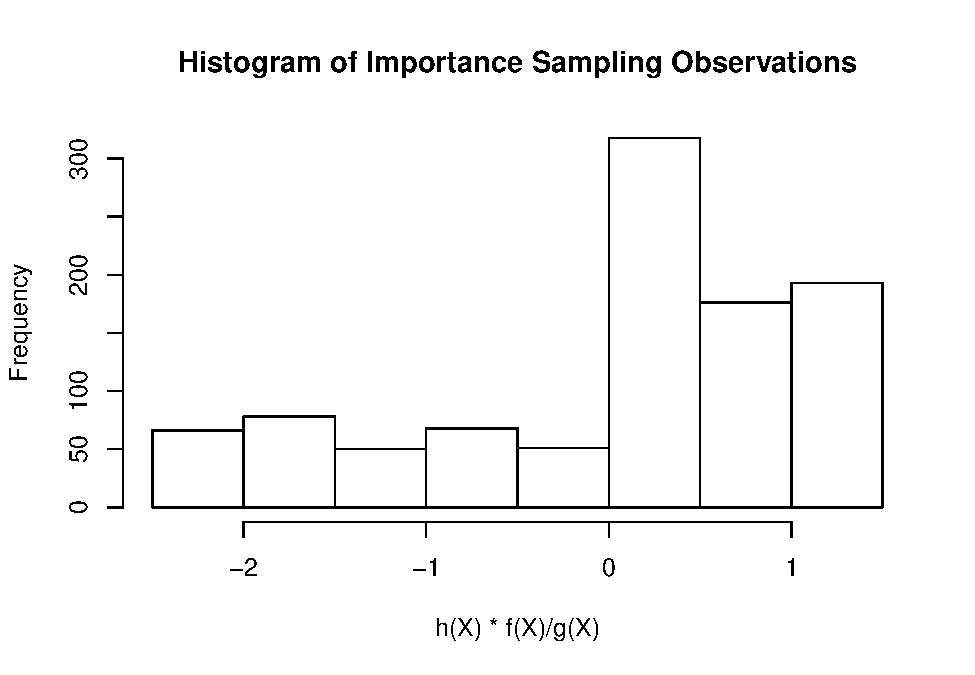
\includegraphics{Atlas-PS_5_files/figure-latex/unnamed-chunk-1-1.pdf}

\begin{Shaded}
\begin{Highlighting}[]
\KeywordTok{hist}\NormalTok{(X_direct, }\DataTypeTok{main=}\StringTok{"Histogram of N(0, 1)"}\NormalTok{, }\DataTypeTok{xlab=}\StringTok{"X"}\NormalTok{)}
\end{Highlighting}
\end{Shaded}

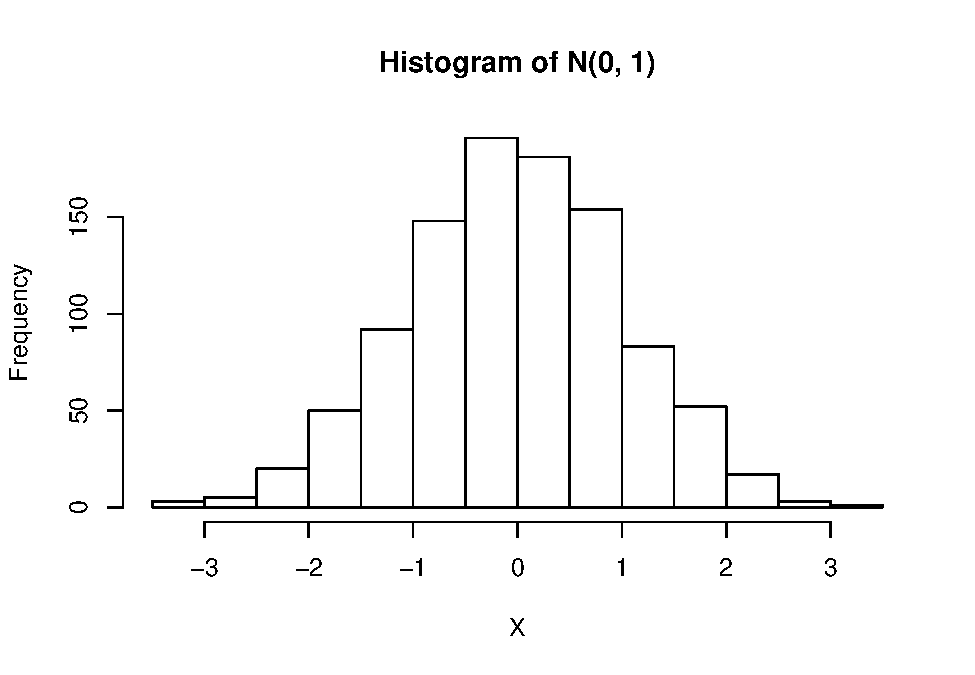
\includegraphics{Atlas-PS_5_files/figure-latex/unnamed-chunk-1-2.pdf}

We see that the weighted mean and variance found via importance sampling
is very close to our target distribution. However, the histogram shows
that the observations themselves do not appear to be normally
distributed.

\section{Problem 3}\label{problem-3}

\subsection{a)}\label{a-1}

We define the transition probability matrix. \[P =
\kbordermatrix{
    \mbox{ } & \textrm{Positive Tomorrow} & \textrm{Negative Tomorrow} & \textrm{It Could Be Worse Tomorrow} \\
   \textrm{Positive Today}& 0                      & .5 & .5 \\
    \textrm{Negative Today} &  .25          & .5 & .25  \\
    \textrm{It Could Be Worse Today} & .25   & .25 & .5
}
\]

\subsection{b)}\label{b-1}

We solve \(\pi P = \pi\) by multiplying the matricies to get the
following system of equations, where the last one enforces the summing
of probabilties to 1.

\begin{align*}
&-\pi_p + .5 \pi_n + .5 \pi_w = 0 \\
&.25\pi_p + -.5 \pi_n + .25 \pi_w = 0 \\
&.25\pi_p + .25 \pi_n + -.5 \pi_w = 0 \\
& \pi_p + \pi_n +\pi_w =1
\end{align*}

We can solve this system of equations using many techniques, but in the
spirit of simulation, we will solve it with the recursive equation
\(\pi_t = \pi_{t-1} P\):

\begin{Shaded}
\begin{Highlighting}[]
\NormalTok{pi0 <-}\StringTok{ }\KeywordTok{c}\NormalTok{(}\DecValTok{1}\NormalTok{/}\DecValTok{3}\NormalTok{, }\DecValTok{1}\NormalTok{/}\DecValTok{3}\NormalTok{, }\DecValTok{1}\NormalTok{/}\DecValTok{3}\NormalTok{)}
\NormalTok{pit <-}\StringTok{ }\KeywordTok{c}\NormalTok{(}\DecValTok{1}\NormalTok{, }\DecValTok{1}\NormalTok{, }\DecValTok{1}\NormalTok{)}
\NormalTok{P <-}\StringTok{  }\KeywordTok{matrix}\NormalTok{(}\KeywordTok{c}\NormalTok{(}\DecValTok{0}\NormalTok{, .}\DecValTok{5}\NormalTok{, .}\DecValTok{5}\NormalTok{, .}\DecValTok{25}\NormalTok{, .}\DecValTok{5}\NormalTok{, .}\DecValTok{25}\NormalTok{, .}\DecValTok{25}\NormalTok{, .}\DecValTok{25}\NormalTok{, .}\DecValTok{5}\NormalTok{), }\DataTypeTok{ncol=}\DecValTok{3}\NormalTok{, }\DataTypeTok{byrow=}\OtherTok{TRUE}\NormalTok{)}
\NormalTok{while (}\KeywordTok{sum}\NormalTok{(}\KeywordTok{abs}\NormalTok{(pi0 -}\StringTok{ }\NormalTok{pit)) >}\StringTok{ }\NormalTok{.}\DecValTok{0001}\NormalTok{)\{}
  \NormalTok{pi0 <-}\StringTok{ }\NormalTok{pit}
  \NormalTok{pit <-}\StringTok{ }\NormalTok{pi0 %*%}\StringTok{ }\NormalTok{P}
\NormalTok{\}}
\NormalTok{solution <-}\StringTok{ }\KeywordTok{data.frame}\NormalTok{(pit %*%}\StringTok{ }\NormalTok{P)}
\KeywordTok{colnames}\NormalTok{(solution) <-}\StringTok{ }\KeywordTok{c}\NormalTok{(}\StringTok{"P"}\NormalTok{, }\StringTok{"N"}\NormalTok{, }\StringTok{"W"}\NormalTok{)}
\CommentTok{# Print the normalized solutions}
\NormalTok{knitr::}\KeywordTok{kable}\NormalTok{(}\KeywordTok{round}\NormalTok{(solution /}\StringTok{ }\KeywordTok{sum}\NormalTok{(solution), }\DecValTok{3}\NormalTok{))}
\end{Highlighting}
\end{Shaded}

\begin{longtable}[]{@{}rrr@{}}
\toprule
P & N & W\tabularnewline
\midrule
\endhead
0.2 & 0.4 & 0.4\tabularnewline
\bottomrule
\end{longtable}

We see that in the long run, 60\% of the time, the general population
will have a non-negative opinion of the government.

\section{Problem 4}\label{problem-4}

\subsection{a)}\label{a-2}

We implement the Metropolis-Hastings Algorithm to generate observations
from a mixing distribution \[
f(x) = \delta N(7, .5^2) + (1 - \delta)N(10, .5^2).
\] We use \[
g(x^* \vert x^{(t)}) = \phi(x^*, x^{(t)}, .01^2)
\] as the proposal density, thereby drawing proposed observations from
\(N(x^{(t)}, .01^2)\).

We use \({0, 7, 15}\) as the set of starting points \(x_0\).

\begin{Shaded}
\begin{Highlighting}[]
\KeywordTok{set.seed}\NormalTok{(}\DecValTok{73}\NormalTok{)}

\CommentTok{# We implement our density functions f and g}
\NormalTok{f <-}\StringTok{ }\NormalTok{function(x, }\DataTypeTok{lambda=}\NormalTok{.}\DecValTok{7}\NormalTok{) lambda *}\StringTok{ }\KeywordTok{dnorm}\NormalTok{(x, }\DecValTok{7}\NormalTok{, .}\DecValTok{5}\NormalTok{^}\DecValTok{2}\NormalTok{) +}\StringTok{ }\NormalTok{(}\DecValTok{1} \NormalTok{-}\StringTok{ }\NormalTok{lambda) *}\StringTok{ }\KeywordTok{dnorm}\NormalTok{(x, }\DecValTok{10}\NormalTok{, .}\DecValTok{5}\NormalTok{^}\DecValTok{2}\NormalTok{)}
\NormalTok{g <-}\StringTok{ }\NormalTok{function(x, x0) }\KeywordTok{dnorm}\NormalTok{(x, }\DataTypeTok{mean=}\NormalTok{x0, }\DataTypeTok{sd=}\NormalTok{.}\DecValTok{01}\NormalTok{^}\DecValTok{2}\NormalTok{)}

\CommentTok{# We implement our random distribution to draw from (the density is g)}
\NormalTok{rg <-}\StringTok{ }\NormalTok{function(x0) }\KeywordTok{rnorm}\NormalTok{(}\DataTypeTok{n=}\DecValTok{1}\NormalTok{, }\DataTypeTok{mean=}\NormalTok{x0, }\DataTypeTok{sd=}\NormalTok{.}\DecValTok{01}\NormalTok{^}\DecValTok{2}\NormalTok{)}

\CommentTok{# Helper function to determine whether or not to keep the random draw}
\NormalTok{find_xt <-}\StringTok{ }\NormalTok{function(xstar, xt, mh_ratio)\{}
  \NormalTok{cutoff <-}\StringTok{ }\KeywordTok{runif}\NormalTok{(}\DataTypeTok{n=}\DecValTok{1}\NormalTok{, }\DataTypeTok{min=}\DecValTok{0}\NormalTok{, }\DataTypeTok{max=}\DecValTok{1}\NormalTok{) }\CommentTok{# Draw from U(0, 1)}
  \KeywordTok{return}\NormalTok{(}\KeywordTok{ifelse}\NormalTok{(cutoff <}\StringTok{ }\KeywordTok{min}\NormalTok{(mh_ratio, }\DecValTok{1}\NormalTok{), xstar, xt)) }
\NormalTok{\}}

\CommentTok{# MH Algorithm }
\NormalTok{metropolis_hastings <-}\StringTok{ }\NormalTok{function(g, rg,  f, x0, }\DataTypeTok{iterations=}\DecValTok{10000}\NormalTok{)\{}
  \NormalTok{path <-}\StringTok{ }\KeywordTok{rep}\NormalTok{(}\DecValTok{0}\NormalTok{, iterations) }\CommentTok{# Vector to hold path}
  
  \CommentTok{# Loop through iterations}
  \NormalTok{for (i in }\DecValTok{1}\NormalTok{:iterations)\{}
    \CommentTok{# Get a random draw from g}
    \NormalTok{xstar <-}\StringTok{ }\KeywordTok{rg}\NormalTok{(x0)}
    
    \CommentTok{# Calculate the MH ratio given the data}
    \NormalTok{mh_ratio <-}\StringTok{ }\NormalTok{(}\KeywordTok{f}\NormalTok{(xstar) *}\StringTok{ }\KeywordTok{g}\NormalTok{(x0, xstar)) /}\StringTok{ }\NormalTok{(}\KeywordTok{f}\NormalTok{(x0) *}\StringTok{ }\KeywordTok{g}\NormalTok{(xstar, x0))}
    
    \CommentTok{# Update the point (using function above)}
    \NormalTok{x0 <-}\StringTok{ }\KeywordTok{find_xt}\NormalTok{(xstar, x0, mh_ratio)}
    
    \CommentTok{# Add the point to the path}
    \NormalTok{path[i] <-}\StringTok{ }\NormalTok{x0}
  \NormalTok{\}}
  \KeywordTok{return}\NormalTok{(path)}
\NormalTok{\}}
\end{Highlighting}
\end{Shaded}

Next, we run the function using each of the starting points.

\begin{Shaded}
\begin{Highlighting}[]
\KeywordTok{set.seed}\NormalTok{(}\DecValTok{73}\NormalTok{)}
\NormalTok{for(i in }\KeywordTok{c}\NormalTok{(}\DecValTok{0}\NormalTok{, }\DecValTok{7}\NormalTok{, }\DecValTok{15}\NormalTok{))\{}
  \NormalTok{path <-}\StringTok{ }\KeywordTok{metropolis_hastings}\NormalTok{(}\DataTypeTok{g=}\NormalTok{g, }\DataTypeTok{rg=}\NormalTok{rg, }\DataTypeTok{f=}\NormalTok{f, }\DataTypeTok{x0=}\NormalTok{i, }\DataTypeTok{iterations=}\DecValTok{10000}\NormalTok{)}
  \KeywordTok{plot}\NormalTok{(}\KeywordTok{seq}\NormalTok{(}\DecValTok{1}\NormalTok{, }\DecValTok{10000}\NormalTok{), path, }\StringTok{'l'}\NormalTok{, }\DataTypeTok{main=}\KeywordTok{paste0}\NormalTok{(}\StringTok{"Starting Point: "}\NormalTok{, i), }
       \DataTypeTok{xlab=}\StringTok{'t'}\NormalTok{, }\DataTypeTok{ylab=}\KeywordTok{TeX}\NormalTok{(}\StringTok{"$x^\{(t)\}$"}\NormalTok{))}
\NormalTok{\}}
\end{Highlighting}
\end{Shaded}

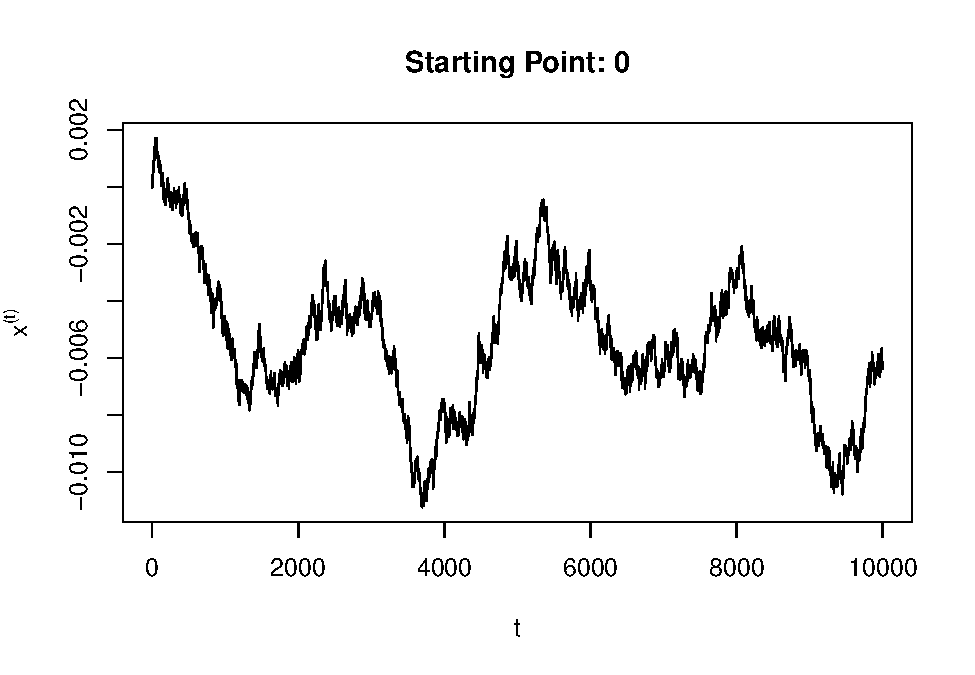
\includegraphics{Atlas-PS_5_files/figure-latex/unnamed-chunk-4-1.pdf}
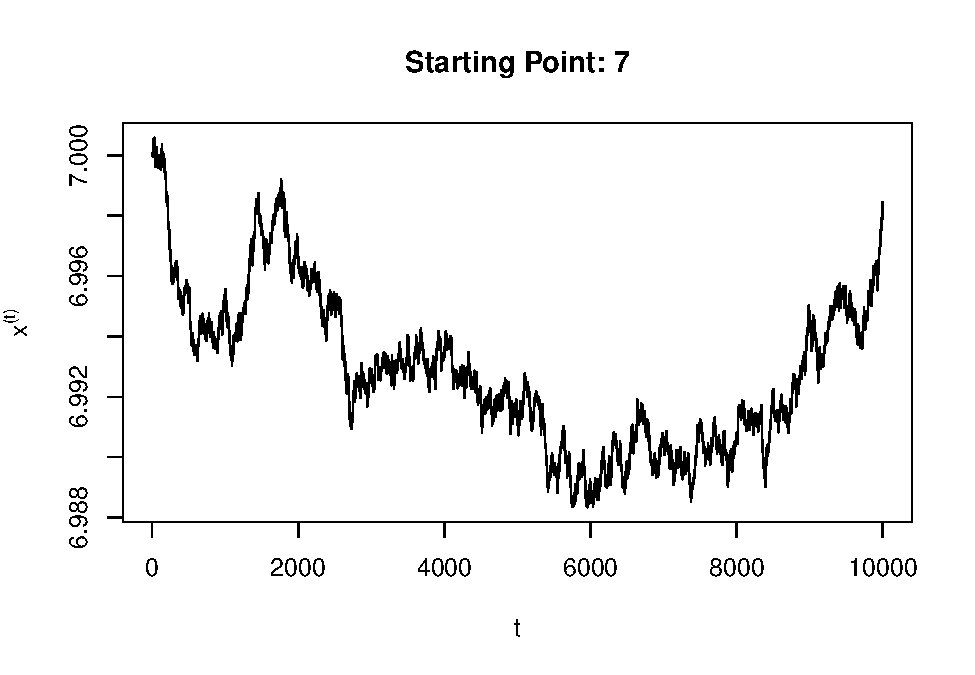
\includegraphics{Atlas-PS_5_files/figure-latex/unnamed-chunk-4-2.pdf}
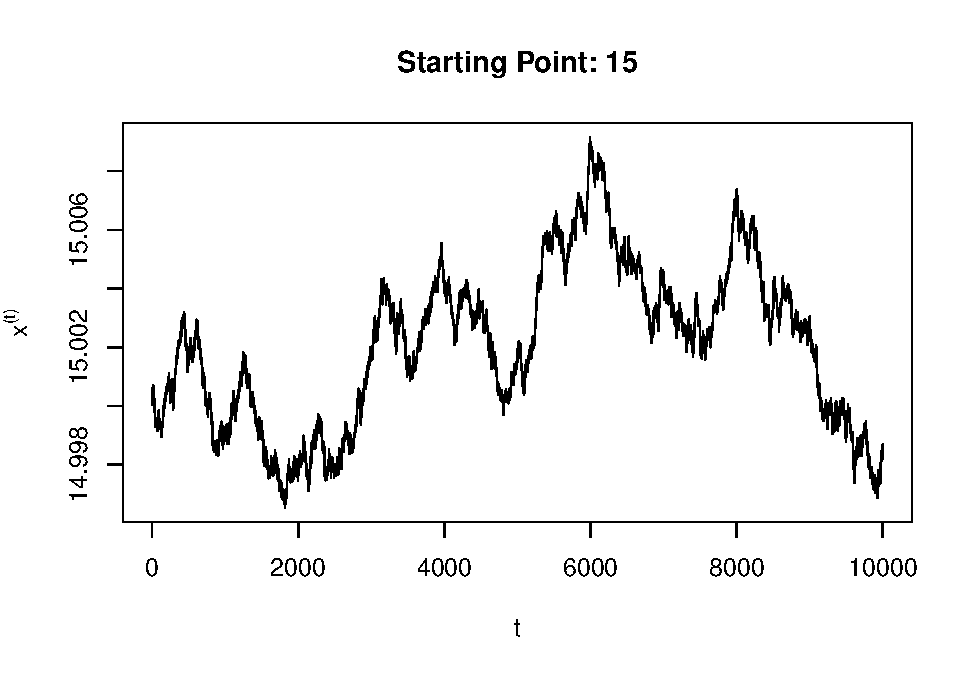
\includegraphics{Atlas-PS_5_files/figure-latex/unnamed-chunk-4-3.pdf}

If only one of the given paths were available, it would be reasonable to
reject the results, as the paths do not appear to have converged within
some bounds. We might try to run more iterations to get a better sample.

Next, we plot the histograms of each of the distributions.

\begin{Shaded}
\begin{Highlighting}[]
\KeywordTok{set.seed}\NormalTok{(}\DecValTok{73}\NormalTok{)}
\NormalTok{for(i in }\KeywordTok{c}\NormalTok{(}\DecValTok{0}\NormalTok{, }\DecValTok{7}\NormalTok{, }\DecValTok{15}\NormalTok{))\{}
  \NormalTok{path <-}\StringTok{ }\KeywordTok{metropolis_hastings}\NormalTok{(}\DataTypeTok{g=}\NormalTok{g, }\DataTypeTok{rg=}\NormalTok{rg, }\DataTypeTok{f=}\NormalTok{f, }\DataTypeTok{x0=}\NormalTok{i, }\DataTypeTok{iterations=}\DecValTok{10000}\NormalTok{)}
  \KeywordTok{hist}\NormalTok{(path, }\DataTypeTok{main=}\KeywordTok{paste0}\NormalTok{(}\StringTok{"Starting Point: "}\NormalTok{, i), }\DataTypeTok{xlab=}\StringTok{'X'}\NormalTok{)}
\NormalTok{\}}
\end{Highlighting}
\end{Shaded}

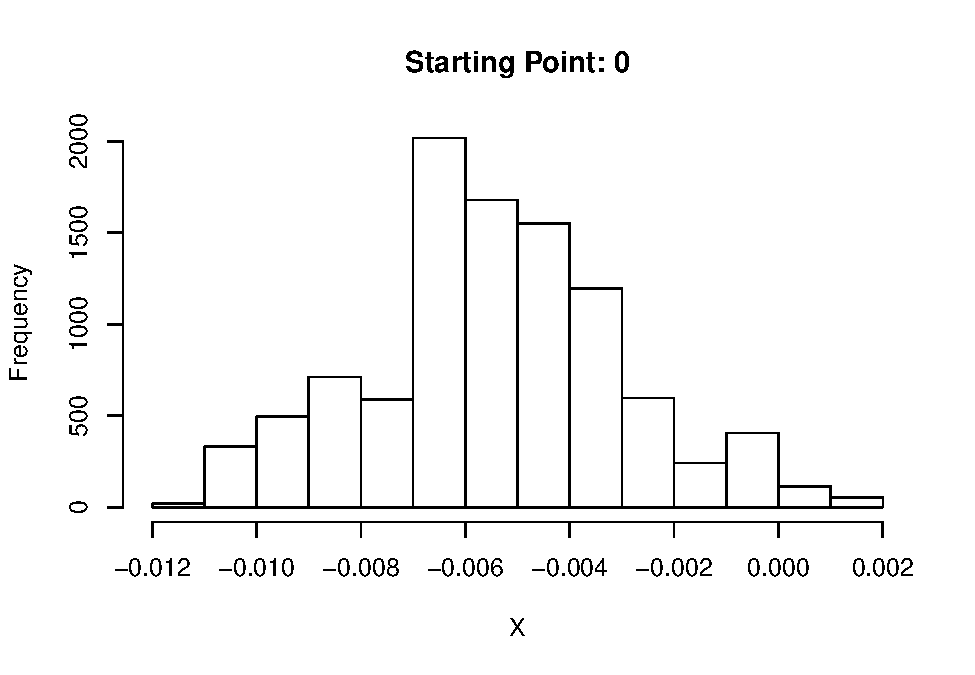
\includegraphics{Atlas-PS_5_files/figure-latex/unnamed-chunk-5-1.pdf}
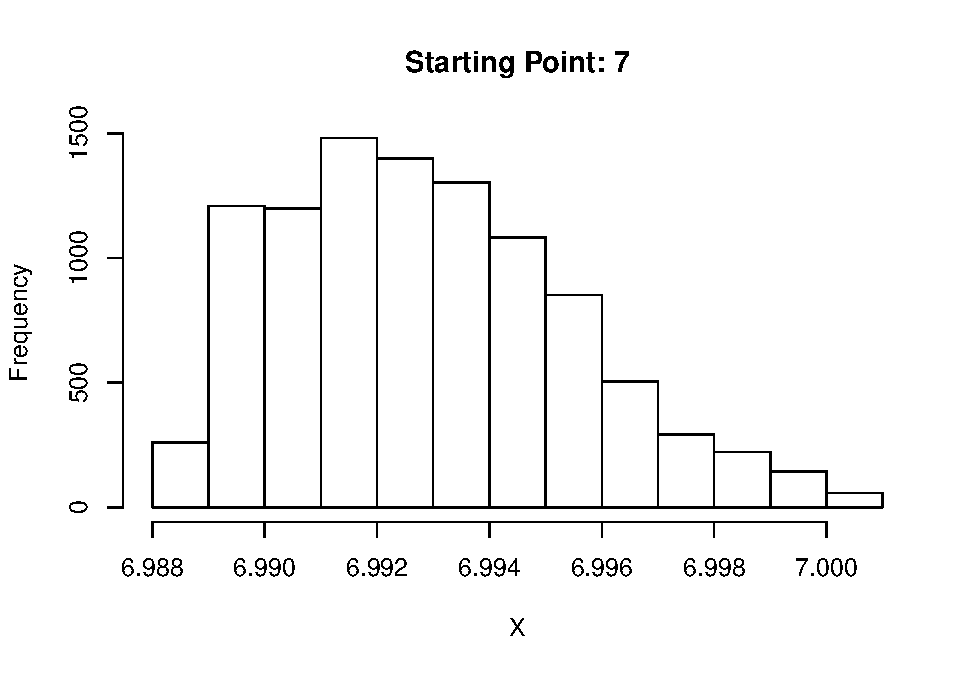
\includegraphics{Atlas-PS_5_files/figure-latex/unnamed-chunk-5-2.pdf}
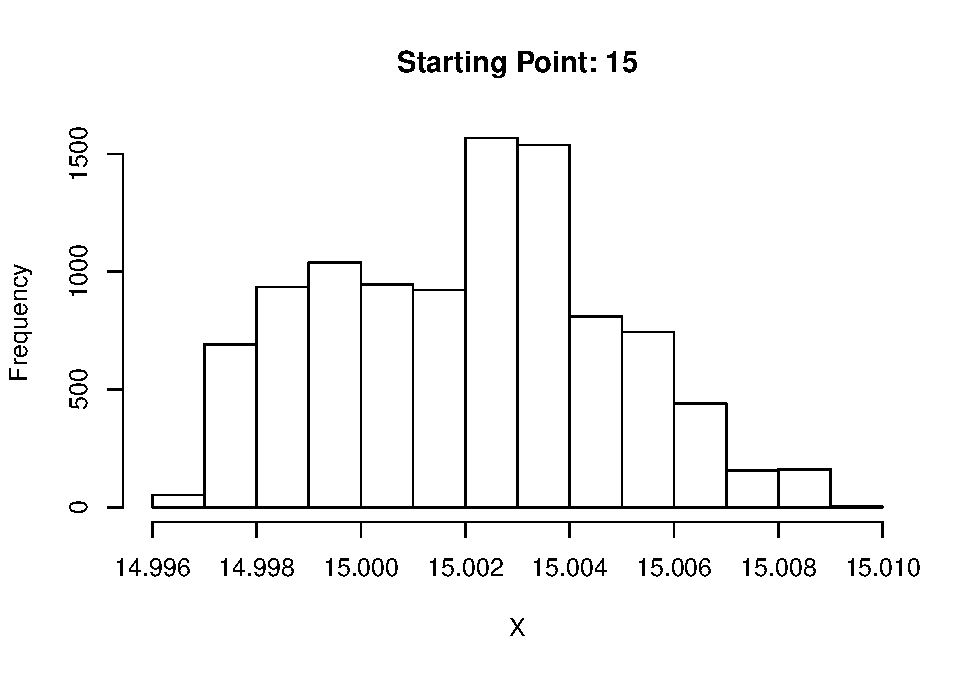
\includegraphics{Atlas-PS_5_files/figure-latex/unnamed-chunk-5-3.pdf}

The histograms have density clustered around the starting value. Based
on all of the paths, it's pretty clear that none of them represent the
true density. Intuitively, it appears that increasing the variance on
the proposal distribution may help, as the simulations are all clustered
very tightly around the starting point, and don't appear to have the
needed variance to sniff out the correct density.

Next, we change our proposal distribution to \(U(0, 20)\) with
\(x_0=7\). We plot the path and the histogram.

\begin{Shaded}
\begin{Highlighting}[]
\CommentTok{# Define proposal distributions}
\NormalTok{g <-}\StringTok{ }\NormalTok{function(xstar, x0) }\KeywordTok{dunif}\NormalTok{(xstar, }\DecValTok{0}\NormalTok{, }\DecValTok{20}\NormalTok{)}
\NormalTok{rg <-}\StringTok{ }\NormalTok{function(x0) }\KeywordTok{runif}\NormalTok{(}\DataTypeTok{n=}\DecValTok{1}\NormalTok{, }\DataTypeTok{min=}\DecValTok{0}\NormalTok{, }\DataTypeTok{max=}\DecValTok{20}\NormalTok{)}

\NormalTok{x0 <-}\StringTok{ }\KeywordTok{c}\NormalTok{(}\DecValTok{7}\NormalTok{)}
\KeywordTok{set.seed}\NormalTok{(}\DecValTok{73}\NormalTok{)}
\NormalTok{for(i in x0)\{}
  \NormalTok{path <-}\StringTok{ }\KeywordTok{metropolis_hastings}\NormalTok{(}\DataTypeTok{g=}\NormalTok{g, }\DataTypeTok{rg=}\NormalTok{rg, }\DataTypeTok{f=}\NormalTok{f, }\DataTypeTok{x0=}\NormalTok{i, }\DataTypeTok{iterations=}\DecValTok{10000}\NormalTok{)}
  \KeywordTok{plot}\NormalTok{(}\KeywordTok{seq}\NormalTok{(}\DecValTok{1}\NormalTok{, }\DecValTok{10000}\NormalTok{), path, }\StringTok{'l'}\NormalTok{, }\DataTypeTok{main=}\KeywordTok{paste0}\NormalTok{(}\StringTok{"Starting Point: "}\NormalTok{, i), }\DataTypeTok{xlab=}\StringTok{'t'}\NormalTok{, }\DataTypeTok{ylab=}\KeywordTok{TeX}\NormalTok{(}\StringTok{"$x^\{(t)\}$"}\NormalTok{))}
  \KeywordTok{hist}\NormalTok{(path, }\DataTypeTok{breaks=}\KeywordTok{seq}\NormalTok{(}\KeywordTok{min}\NormalTok{(path) -}\StringTok{ }\NormalTok{.}\DecValTok{1}\NormalTok{, }\KeywordTok{max}\NormalTok{(path) +}\StringTok{ }\NormalTok{.}\DecValTok{1}\NormalTok{, .}\DecValTok{1}\NormalTok{), }\DataTypeTok{main=}\KeywordTok{paste0}\NormalTok{(}\StringTok{"Starting Point: "}\NormalTok{, i), }\DataTypeTok{xlab=}\StringTok{'X'}\NormalTok{, }\DataTypeTok{freq=}\NormalTok{F, }\DataTypeTok{ylim=}\KeywordTok{c}\NormalTok{(}\DecValTok{0}\NormalTok{, }\FloatTok{1.5}\NormalTok{))}
  \KeywordTok{lines}\NormalTok{(}\KeywordTok{seq}\NormalTok{(}\KeywordTok{min}\NormalTok{(path), }\KeywordTok{max}\NormalTok{(path), .}\DecValTok{01}\NormalTok{), }\KeywordTok{f}\NormalTok{(}\KeywordTok{seq}\NormalTok{(}\KeywordTok{min}\NormalTok{(path), }\KeywordTok{max}\NormalTok{(path), .}\DecValTok{01}\NormalTok{)))}
\NormalTok{\}}
\end{Highlighting}
\end{Shaded}

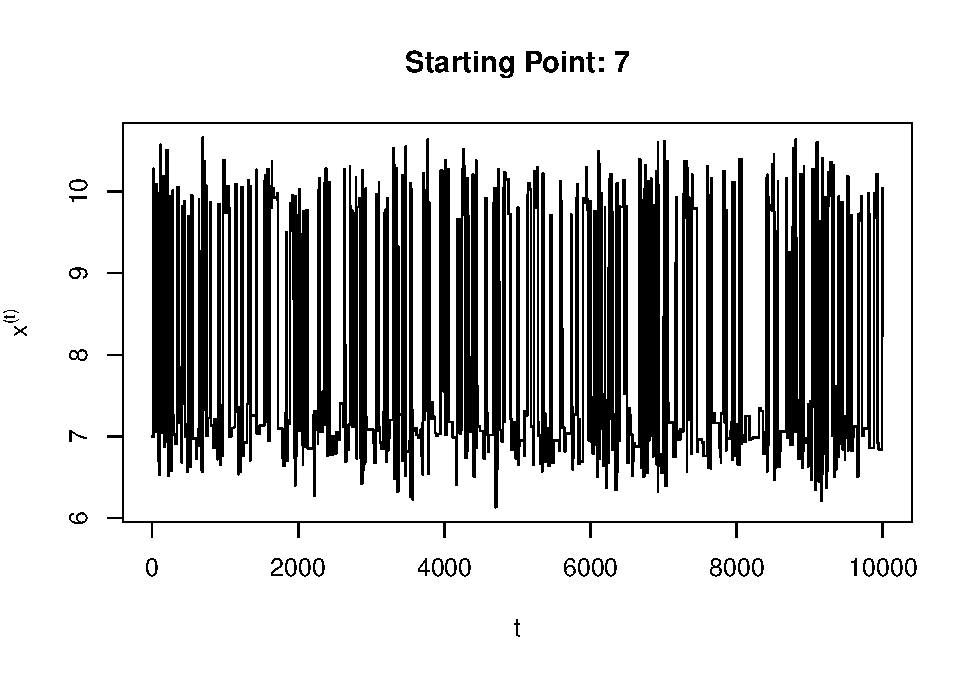
\includegraphics{Atlas-PS_5_files/figure-latex/unnamed-chunk-6-1.pdf}
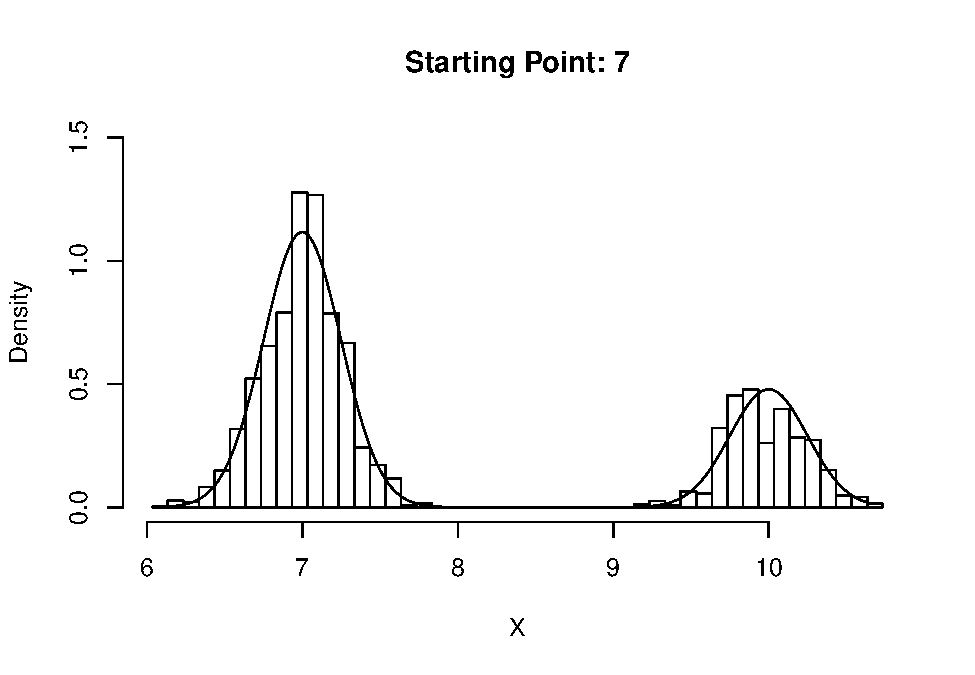
\includegraphics{Atlas-PS_5_files/figure-latex/unnamed-chunk-6-2.pdf}

Using the uniform distribution given, our histogram looks correct, based
on our definition for \(f(x)\) (superimposed on the histogram). Also, in
looking at the path given by the MH Algorithm, we note that this appears
to be pretty clearly a mixture of two distributions with different
means, as the path alternates between the two means with a very regular
pattern.


\end{document}
